\section{Versuchsaufbau: LEP und OPAL}
Im Versuch werden Daten ausgewertet, die in den Jahren 1989 bis 2000 am
CERN\footnote{Conseil Européen pour la Recherche Nucléaire} während des
LEP\footnote{Large Electron-Positron Collider}-Experiments gewonnen wurden.
In dem 27\,km langen Tunnel des Teilchenbeschleunigers wurden Pakete von 
Elektronen und Positronen gegenläufig auf einer Kreisbahn beschleunigt
und kollidierten an vier Stellen im Strahl \cite{manual}.
An jeder der vier Wechselwirkungszonen stand ein Detektor, einer davon war der
OPAL\footnote{Omni Purpose Apparatus at LEP}-Detektor.
Der Aufbau dieses Detektors ist auf \autoref{img:aufbau} gezeigt und wird im Folgenden beschrieben.

\begin{figure}[H]
\begin{center}
  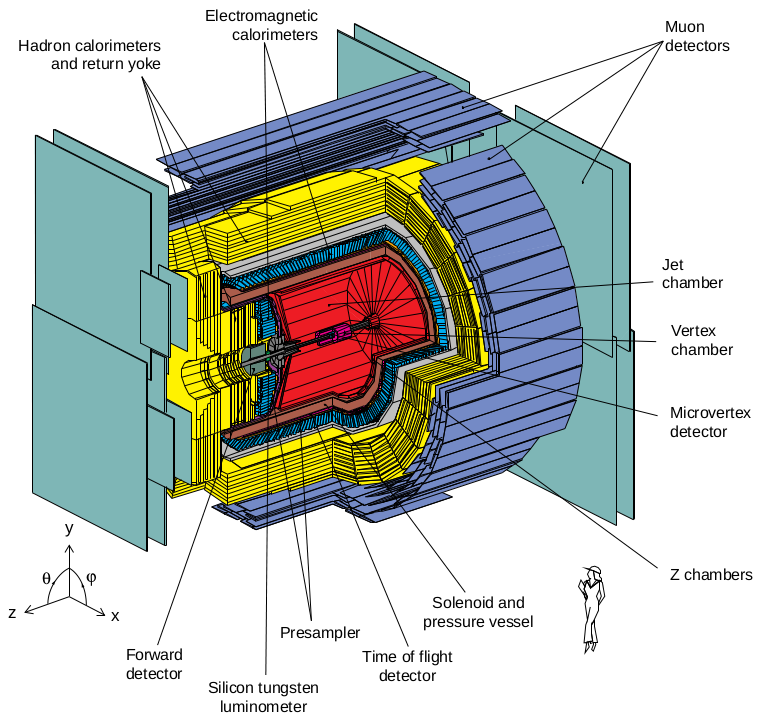
\includegraphics[width=\textwidth]{../img/aufbau.png}
  \caption{Aufbau des OPAL-Detektors am LEP (aus \cite{manualmuc}).}
  \label{img:aufbau}
\end{center}
\end{figure}

\autoref{img:schnitt} zeigt schematisch den groben Aufbau des Detektors:
In unmittelbarer Nähe zum Strahl befinden sich \emph{Spurdetektoren},
mit denen die Bahnkurven der Zerfallsprodukte beobachtet werden.
Anschließend folgen \emph{Kalorimeter} zur Energiemessung und außen ganz außen \emph{Myonendetektoren}.  
%TODO Luminosität

\begin{figure}[H]
\begin{center}
  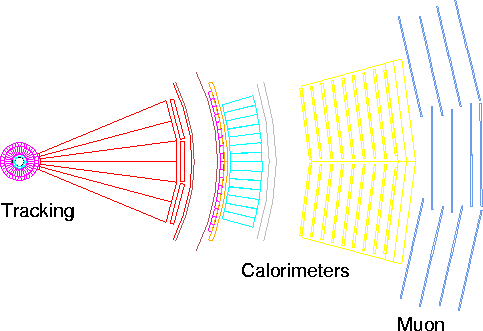
\includegraphics[width=0.55\textwidth]{../img/opalslice_tr.png}
  \caption{Schematischer Schnitt durch den OPAL-Detektor senkrecht zum \mbox{\ee-Strahl}\protect\footnotemark.}
  \label{img:schnitt}
\end{center}
\end{figure} 
\footnotetext{von http://opal.web.cern.ch/Opal/tour/layers.html, aufgerufen am 14.5.2015.}

\subsection*{Spurdetektoren}
Die Detektion der Teilchenspuren erfolgt nach dem Prinzip des Zählrohrs:
Hochenergetische Teilchen erzeugen in einem Gas durch Ionisation freie Elektronen,
die in einem elektrischen Feld zu einer Draht-Anode beschleunigt werden und
dort lawinenartig weitere Atome ionisieren.

Spurdetektoren enthalten sehr viele Drähte mit kleinem Abstand,
so dass eine Rekonstruktion der Flugbahnen der Teilchen möglich ist.
In den Spurdetektoren herrscht ein starkes Magnetfeld,
damit die auftretende Lorentzkraft die Flugbahnen der geladenen Teilchen krümmt
und durch Messung des Krümmungsradius der Teilchenimpuls bestimmt werden kann.

\subsection*{Kalorimeter}
In den Kalorimetern wechselwirken die einfallenden Teilchen mit dem Material des Zählers
und erzeugen ein Signal proportional zu ihrer Energie.
In den Kalorimetern sind abwechselnd Absorptionsmaterial und Detektoren (Szintillatoren) verbaut.

Im ersten, \emph{elektromagnetischen Kalorimeter} wird von Photonen und Elektronen Brems\-strah\-lung erzeugt
und es werden \mbox{\ee-Paare} gebildet.
Im folgenden \emph{hadronischen Kalorimeter} entsteht ein Schauer durch eine Serie von inelastischen Kernstößen
von primären Hadronen mit dem Absorber.

\subsection*{Myon-Detektor}
Den Kalorimetern folgt ein Detektor für Myonen, die aufgrund ihrer geringen Wechselwirkungswahrscheinlichkeit
von den Kalorimetern nicht gestoppt werden.

